\documentclass[draftclsnofoot, onecolumn, compsoc, 10pt]{IEEEtran}

\title{\huge Software Requirements Specifications}
\author{Oregon State University\\CS 461\\2017-2018\\\\Prepared By:\\ Kyle Prouty\\Hayden Anderson\\}
\usepackage{lscape}
\usepackage{rotating}
\usepackage{titling}
\usepackage[margin=0.75in]{geometry}
\usepackage{graphicx}
\usepackage{placeins}
\usepackage{url}
\usepackage{setspace}
\geometry{textheight=9.5in, textwidth=7in}
\graphicspath{ {images/} }
\linespread{1.0}
\parindent=0.0in
\parskip=0.2in


% 1. Fill in these details
\def \CapstoneTeamName{		Rodents Of Unusual Size}
\def \CapstoneTeamNumber{		46}
\def \GroupMemberOne{			Hayden Anderson}
\def \GroupMemberTwo{			Kyle Prouty}
\def \CapstoneProjectName{		Project ROUS}
\def \CapstoneSponsorCompany{	HP, Inc}
\def \CapstoneSponsorPerson{	Lonnie Mandigo}

% 2. Uncomment the appropriate line below so that the document type works
\def \DocType{  %Problem Statement
				Requirements Document
				%Technology Review
				%Design Document
				%Progress Report
				}
			
\newcommand{\NameSigPair}[1]{\par
\makebox[2.75in][r]{#1} \hfil 	\makebox[3.25in]{\makebox[2.25in]{\hrulefill} \hfill		\makebox[.75in]{\hrulefill}}
\par\vspace{-12pt} \textit{\tiny\noindent
\makebox[2.75in]{} \hfil		\makebox[3.25in]{\makebox[2.25in][r]{Signature} \hfill	\makebox[.75in][r]{Date}}}}
% 3. If the document is not to be signed, uncomment the RENEWcommand below
%\renewcommand{\NameSigPair}[1]{#1}

%%%%%%%%%%%%%%%%%%%%%%%%%%%%%%%%%%%%%%%
\begin{document}
\begin{titlepage}
    \pagenumbering{gobble}
    \begin{singlespace}
%     	\includegraphics[height=4cm]{coe_v_spot1}
        \hfill 
        % 4. If you have a logo, use this includegraphics command to put it on the coversheet.
        %\includegraphics[height=4cm]{CompanyLogo}   
        \par\vspace{.2in}
        \centering
        \scshape{
            \huge CS Capstone \DocType \par
            {\large\today}\par
            \vspace{.5in}
            \textbf{\Huge\CapstoneProjectName}\par
            \vfill
            {\large Prepared for}\par
            \Huge \CapstoneSponsorCompany\par
            \vspace{5pt}
            {\Large\NameSigPair{\CapstoneSponsorPerson}\par}
            {\large Prepared by }\par
            Group\CapstoneTeamNumber\par
            % 5. comment out the line below this one if you do not wish to name your team
            \CapstoneTeamName\par 
            \vspace{5pt}
            {\Large
                \NameSigPair{\GroupMemberOne}\par
                \NameSigPair{\GroupMemberTwo}\par
            }
            \vspace{20pt}
        }
        \begin{abstract}
        This document will give an overview of software dependencies, the intended function, characteristics, constraints, and assumptions of the framework. The first section is geared more towards giving a more high level examination of the framework. The third and fourth sections, Specific Requirements and Software System Attributes, is intended for more of a technical audience who would be familiar with the technical aspects and relevant terminology of this framework.  
        \end{abstract}     
    \end{singlespace}
\end{titlepage}
\newpage
\pagenumbering{arabic}
\clearpage 
\tableofcontents
\pagebreak



\section{Introduction}
\subsection{Purpose} 
The purpose of this document is to layout and define the objective and details of the framework to be developed. This document will specify an overall description, specific requirements, and software system attributes of this framework. The intended audience for this document includes any relevant stakeholders. This document details what the project's end product will do for an end user.

\subsection{Scope}
This main purpose of this framework will be to allow a user to input an objective into a collection of nodes, see the nodes organize on that object, and then see the result of that organization. Nodes will carryout an objective based on the services available. Three main goals will be achieved in order to complete the main objective. First, the framework will enable nodes to communicate with each other and will have the ability to share processes. Next, an objective will be able to be inputed into the framework. Finally, the nodes will self organize on the objective and output the results to the user.
% The services needed to finish the job will propagate through the system to find the nodes that can carryout each service. Once each service in an objective has a node that can carry them out. The node that received the user input will output where the piece(s) of the objective are being completed. The framework will be able to (re)direct services and jobs away from established security threatened nodes.  
% \centering{
% 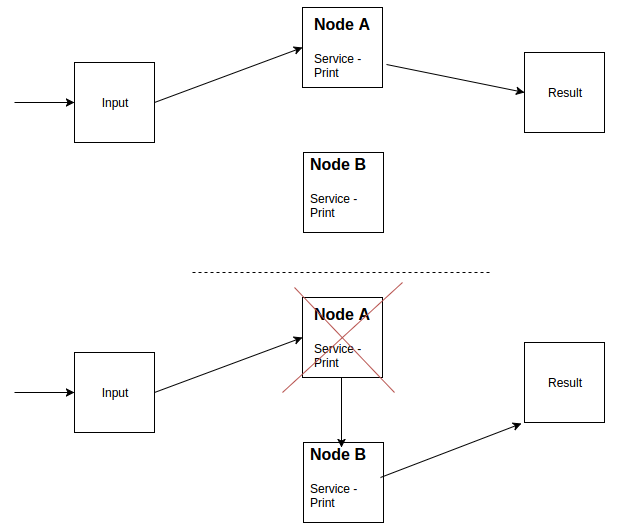
\includegraphics[scale=0.4]{img_1}
% }

\subsection{Definitions, Acronyms, Abbreviations}
\bgroup
\def\arraystretch{1.5}
\resizebox{\textwidth}{!}{
\begin{tabular}{| p{10.0cm} | p{10.0cm} |}
\hline
\bf{Term} & \bf{Definition}\\ 
\hline
Stakeholder  & User of the framework \\
\hline
User  & The person who would use this at its completion that doesn’t know how it works   \\
\hline
Node  & Our built device that acts as a layer between IoT enabled machines and other nodes \\ 
\hline
Docker &  A container of isolated code \\
\hline
Unix & An open-source operating system \\
\hline
Rodents of Unusual Size (ROUS)  &  Project name  \\ 
\hline
Graphical User Interface (GUI)  & A visual representation for the user to interact with  \\ 
\hline
Internet of Things (IoT)  & A blanket statement to describe objects that have been made to be able to connect to the Internet.  \\ 
\hline
Model View Controller (MVC)  &  A software architecture for implementing an interface for the user  \\ 
\hline
Local Area Network (LAN) & A network of connected devices contained within a small geographical space  \\
\hline
Message Queue Telemetry Transport (MQTT) & lightweight TCP/IP protocol\\
\hline
Advanced RISC Machine (ARM) architecture & computer processor architecture \\
\hline
\end{tabular}
}
\egroup

\subsection{References}
IEEE. IEEE Std 830-1998 IEEE Recommended Practice for Software Requirements Specifications. IEEE Computer Society,1998.

\subsection{Overview}
In the next section of this document, Overall Description, will give an overview of software dependencies, the intended function, characteristics, constraints, and assumptions of the framework. This section is geared more towards giving a more high level examination of the framework. The third and fourth sections, Specific Requirements and Software System Attributes, is intended for more of a technical audience who would be familiar with the technical aspects and relevant terminology of this framework. 

\section{Overall Description}
\subsection{Product Perspective}
The framework is designed to offer services that will interact with outside systems. It will act as a middle layer between a user and the outside system. An example of an outside system is a printer. 
\begin{figure}[!htb]
\centering
	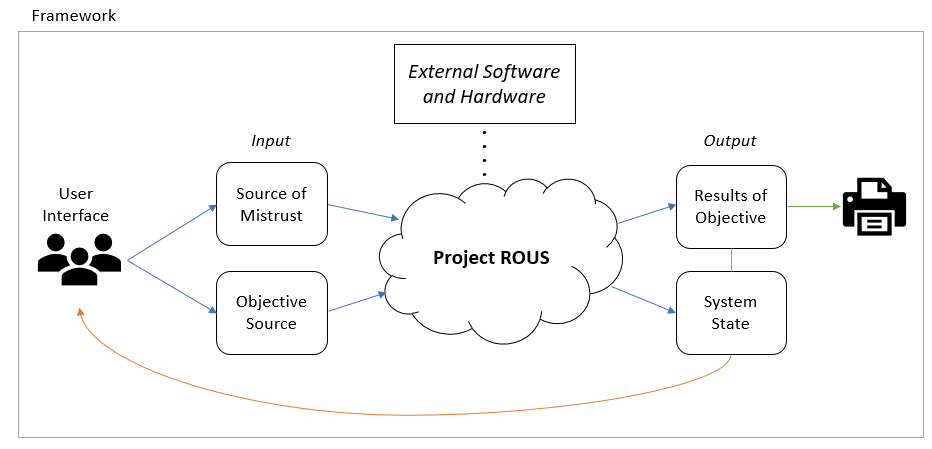
\includegraphics[width=0.7\textwidth]{img_perspective2}
	\caption{This figure shows an objective being inputed into the system, the framework receiving the objective and then organizing on that objective. Next the data is sent to the proper service, and finally the result.}
  
\end{figure}

\subsubsection{System Interfaces}
The primary system interface will be a Unix based operating system. This framework will interact with the Unix operating system in order to utilize its services. 

\subsubsection{User Interfaces}
\begin{itemize}
\item A command line based interface used to connect to a specific node to change configuration setting.\\
\item A web based gui that will interface between an administrator and the nodes. This graphical interface is used to show the nodes in the framework, the services each node offers, and the nodes connections with each other.\\ 
\item A web based gui that will interface between a user and the nodes. This graphical interface is used to let a user upload a file into the collection of nodes and view the status of the result.
\end{itemize}

\subsubsection{Hardware Interfaces}
This framework will use a combination of various ARM based micro-controllers. These micro-controllers must have the functionality to communicate with 802.11 b/g/n wireless LAN communication protocols.

\subsubsection{Software Interfaces}
Nodes will only interact with the Unix based operating system. Users will interact with a web based browser.

\subsubsection{Communications Interfaces}
The network protocol that is required by this framework is Ethernet, with communication protocols TCP/IP and 802.11 b/g/n wireless LAN.

\subsubsection{Memory constraints}
The framework is only constrained to what the hardware that is used will allow.
 
\subsubsection{Operations}
There will be three modes of operation within the user organization. 
\begin{itemize}
\item Node Operation Mode \\
\item User Mode \\ 
\item Administrator Mode
\end{itemize}
The main mode of operation is the node operation mode. This mode will operate exclusively in the background. Next is the user mode which will be input and output operations. Third there will be an administer mode which will allow the sending of commands and the viewing of state and status operations.

\subsubsection{Site Adaptation Requirements}
There are no site adaptations required.


\subsection{Product Functions}
%intro blurb
\begin{itemize}
\item A user interface to send an objective to the framework
\item A user interface to visual see the results of sending an objective to the framework.
\item An administrator interface to send commands to the framework
\item An administrator interface that will show available services offered by each node
\item An administrator interface that will show the state of the framework
\item A command that will block services on a specific node
\item A command that will shutdown services
\item A node will get information about other nodes on the network
\item A node will offer a print service
\item A node will share processes with other nodes
\item A node will keep a memory of tasks sent from user
\item A node will be able to share tasks will other nodes
\end{itemize}
The figure below shows an objective being input into the framework and its corresponding result. Next it shows the same objective going to the same node in the framework but this time the nodes have to self organize and reroute the objective to a different node which achieves the same result.
\begin{figure}[!htb]
  
  \centering
    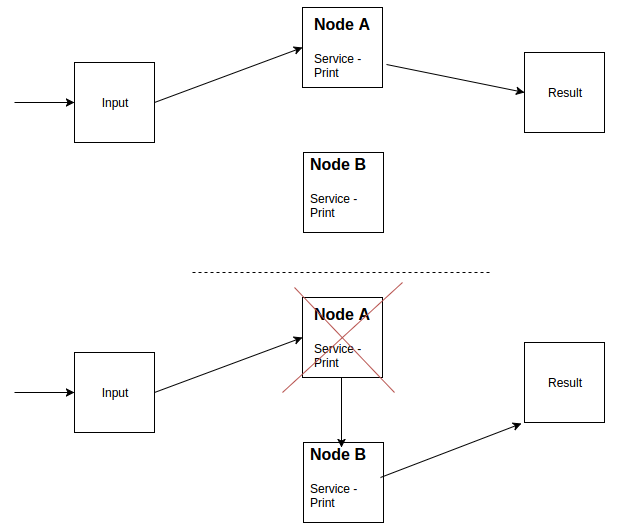
\includegraphics[width=0.5\textwidth]{img_1}
  \caption{Basic description of how this framework will function. }
\end{figure}
\FloatBarrier

\subsection{User Characteristics} 
The users of this framework will be our relevant stakeholders. These users will have had some level of formal technical education.

\subsection{Constraints}
This framework will not communicate to outside sources for any of its configuration settings. Each individual node must be able to lead the framework on decisions required. Nodes cannot utilize an external database for its inner information structure. Nodes cannot exchange information by using an external database.

\subsection{Assumptions and Dependencies}
This document and current requirements assume that each hardware device we use can handle concurrency and has wifi capabilities. Each device has the memory and storage large enough to fit our docker image and run. Each physical device is able to handle a small simple gui.

\subsection{Apportioning of Requirements}
Refer to Gantt chart in figure below for this information.
\begin{landscape}
	\begin{figure}[!htb]
		\caption{Gantt Chart}
		\centering
			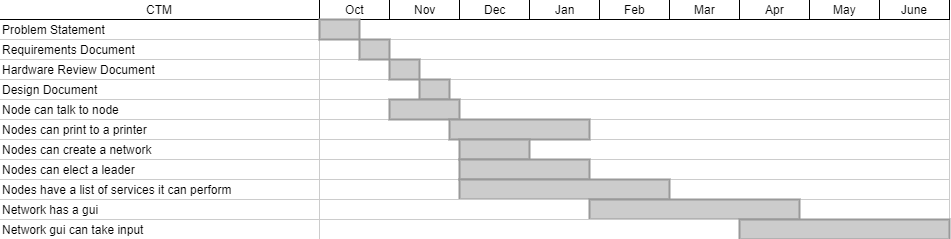
\includegraphics[scale=.7]{chart}
	\end{figure}
\end{landscape}
\FloatBarrier

\section{Specific Requirements}
\subsection{External Interfaces}
\begin{itemize}
\item Input:
	\begin{itemize}
	\item User objectives
    \item Administrator commands
    \item Node operation configuration commands
	\end{itemize}
\item Output:
	\begin{itemize}
	\item Results of inputed objectives
    \item Services
    \item State and configuration data 
	\end{itemize}
\end{itemize}

\subsection{Functions}
The system shall ...
\begin{itemize}
\item Enable nodes to self organize on an inputed objective
\item Allow an objective to be inputed
\item Output readable configuration data
\item Output readable service and state data
\item Automatically validate and connect to authorized nodes
\item Allow nodes to share tasks and processes with each other
\item Allow services to be disabled 
\item Allow services to be shutdown
\item Offer a print service
\end{itemize}

\subsection{Performance Requirements}
This framework will support at a minimum two nodes. Each objective received by the framework from the user will start and execute on 90\% of the services required by the objective given. Only one user will be able to input an objective at a time. Only one objective can be handled by the network at a time. Objectives can be queued and executed consecutively. Each node will support, at a minimum, a print service. A user will have to wait for an objective to complete before inputing a new objective. 

\subsection{Logical Database Requirements}
There are no database requirements. 

\subsection{Design Constraints}
There is not an external database to which the nodes should be writing to or retrieving from to be able to be a part of the nodal network or carry out objectives. The network must be able to send a parallel job to two monochrome printers. The network must be able to send a singular job to a color printer with parallel being a stretch goal.

\subsection{Standards Compliance}
This framework will need to stay compliant with IEEE WLAN and MQTT standards.

%Tell me what you think of the image(Product Perspective), what changes you would make?

%I like it. I think Interface should be capitalized though



\section{Software System Attributes}
\subsection{Reliability}
The reliability of this framework will be measured by the ability to connect to each other, send commands to each other, and view the results of each objective. The nodes will be able to connect and join 8 out of 10 times while also within 20 seconds and within a 10 yard range of an established node. Each sent command will be successful 8 out of 10 times given.

\subsection{Security}
The framework will only accept authorized nodes. Nodes will be password protected and will only accept configuration settings and commands from verified users.

\subsection{Maintainability}
Code will be well commented and readable to 8 out of 10 software developers. A MVC design scheme will be implemented. File structure will be well organized and self explanatory to navigate.


\subsection{Portability}
This framework will be fully portable to any system that can run a Docker container. 

\subsection{Other Requirements}
No additional requirements for this framework.

\end{document}